% !TeX program = xelatex
\documentclass[final, survey]{cpecmu}

%% This is a sample document demonstrating how to use the CPECMU
%% project template. If you are having trouble, see "cpecmu.pdf" for
%% documentation.

\projectNo{P069-1}
\acadyear{2025}

\titleTH{ระบบโหวตความปลอดภัยสูงโดยใช้การกระจายคีย์แบบควอนตัม}
\titleEN{Super-Secure Voting System Using Quantum Key Distribution}

\author{นายภคิน นิรมิตสีมา}{Pakin Niramitsima}{660610782}
\author{นายยุทธกานต์ สาจุ้ย}{Yutthakarn Sajui}{660610787}
\author{นายอาทินันท์ แจ้งสว่าง}{Arthinan Chaengsawang}{660610807}
\author{นายไพสิฐ เลิศอนันต์พิพัฒน์}{Paisit Lerdananpipat}{660612155}

\cpeadvisor{sanpawat}
\cpecommittee{navadon}
\cpecommittee{santi}

\committee{ผศ.ดร.\,วรานนท์ อนุกูล}{Asst.\,Prof.\,Waranont Anukool, Ph.D.}

%% Some possible packages to include:
\usepackage[final]{graphicx} % for including graphics

%% Add bookmarks and hyperlinks in the document.
\PassOptionsToPackage{hyphens}{url}
\usepackage[colorlinks=true,allcolors=Blue4,citecolor=red,linktoc=all]{hyperref}
\def\UrlLeft#1\UrlRight{$#1$}

%% Needed just by this example, but maybe not by most reports
\usepackage{afterpage} % for outputting
\usepackage{pdflscape} % for landscape figures and tables. 

%% Some other useful packages. Look these up to find out how to use
%% them.
% \usepackage{natbib}    % for author-year citation styles
% \usepackage{txfonts}
% \usepackage{appendix}  % for appendices on a per-chapter basis
% \usepackage{xtab}      % for tables that go over multiple pages
% \usepackage{subfigure} % for subfigures within a figure
% \usepackage{pstricks,pdftricks} % for access to special PostScript and PDF commands
% \usepackage{nomencl}   % if you have a list of abbreviations

%% if you're having problems with overfull boxes, you may need to increase
%% the tolerance to 9999
% \tolerance=9999

\bibliographystyle{plain}
% \bibliographystyle{IEEEbib}

% \renewcommand{\topfraction}{0.85}
% \renewcommand{\textfraction}{0.1}
% \renewcommand{\floatpagefraction}{0.75}

%% Example for glossary entry
%% Need to use glossary option
%% See glossaries package for complete documentation.
\ifglossary
  \newglossaryentry{lorem ipsum}{
    name=lorem ipsum,
    description={derived from Latin dolorem ipsum, translated as ``pain itself''}
  }
\fi

%% Uncomment this command to preview only specified LaTeX file(s)
%% imported with \include command below.
%% Any other file imported via \include but not specified here will not
%% be previewed.
%% Useful if your report is large, as you might not want to build
%% the entire file when editing a certain part of your report.
% \includeonly{chapters/intro,chapters/background}

\begin{document}
\include{chapters/frontmatter}

\pagestyle{empty}\cleardoublepage
\normalspacing \setcounter{page}{1} \pagenumbering{arabic} \pagestyle{cpecmu}

\chapter{\ifenglish Introduction\else บทนำ\fi}

\section{\ifenglish Project rationale\else ที่มาของโครงงาน\fi}
ในปัจจุบัน การโหวตนั้นเป็นสิ่งที่พบเห็นได้ทั่วไปเนื่องจากว่าประเทศไทยนั้นมีการปกครองแบบประชาธิปไตร แต่ว่าปัญหาในการโหวตนั้นมีให้เห็นอยู่มากมายเช่น บัตรเสีย การนับคะแนนที่ผิดพลาด
แต่หากเรามาดูรูปแบบการแก้ปัญหาก็พบว่ามีการนำเครื่องเลือกตั้งแบบอิเล็กโทรนิคมาใช้แต่ว่าปัญหาของมันก็คือการที่มีความเสี่ยงจะถูกโจมตีจาก Man-in-the-Middle (MITM) พอมาดูรูปแบบการโหวตต่อไปก็คือการลงคะแนนเสียงออนไลน์ ซึ่งมีความปลอดภัยสูงเพราะว่ามีการเข้ารหัสแบบ RSA ซึ่งเป็นการเข้ารหัสแบบ Asymmetric Encryption แต่ว่าการมาถึงของ
ควอนตัมคอมพิวเตอร์นั้นจะทำให้ การเข้ารหัสแบบนี้ไม่ปลอดภัยเนื่องจากว่าควอนตัมคอมพิวเตอร์นั้นสามารถรัน Shor's algorithm ได้ทำให้การโหวตแบบออนไลน์นั้นไม่ปลอดภัย โครงงานวิจัยเราจึงจัดทำขึ้นเพื่อนำเสนอการส่ง key โดยใช้งาน Quantum Key Distribution (QKD) ในการส่ง key โดยเราจะทำการเข้ารหัสผลการเลือกตั้งเป็นแบบ Symmetric Encryption จากนั้นเราก็จะทำการส่ง key ผ่านทาง Quantum Key Distribution (QKD) ซึ่งรูปแบบนี้เป็นวิธีที่ปลอดภัยต่อการมาถึงของเครื่องควอนตัมคอมพิวเตอร์เพราะว่าคุณสมบัติของควอนตัมนั้นไม่สามารถทำซ้ำได้หากมีการดักฟังก็จะทำให้ผลลัพธ์เปลี่ยน

\section{\ifenglish Objectives\else วัตถุประสงค์ของโครงงาน\fi}
\begin{enumerate}
    \item เพื่อประยุกต์การใช้งาน Quantum Key Distribution ในการส่ง key
    \item เพื่อจำลองการโหวตโดยใช้ควอนตัมคอมพิวเตอร์โดยมีสถานการคือส่งได้แบบปกติและกำลัง
ถูกดักฟัง
\end{enumerate}

\section{\ifenglish Project scope\else ขอบเขตของโครงงาน\fi}

\subsection{\ifenglish Hardware scope\else ขอบเขตด้านฮาร์ดแวร์\fi}
เนื่องจากว่าควอนตัมคอมพิวเตอร์นั้นยังไม่ได้มีการใช้งานอย่างแพร่หลาย เราจึงใช้เครื่องคอมพิวเตอร์ทั่วไปที่สามารถต่ออินเทอร์เน็ตได้ในการเข้าถึงเครื่องควอนตัมคอมพิวเตอร์

\subsection{\ifenglish Software scope\else ขอบเขตด้านซอฟต์แวร์\fi}
จากข้อที่ผ่านมาได้กล่าวว่ายังไม่มีเครื่องควอนตัมคอมพิวเตอร์ในการใช้งาน เราจึงต้องมีการใช้งานแพลตฟอร์ม Quantum Simulation ในออนไลน์ เช่น IBM Quantum และได้มีการใช้งาน ibrary qiskit\_ibm\_runtime ของ Python เพื่อเขียนโปรแกรม Quantum Assembly 

\section{\ifenglish Expected outcomes\else ประโยชน์ที่ได้รับ\fi}
\begin{enumerate}
    \item  ได้ใช้ความรู้เกี่ยวกับการเข้ารห้สแบบ Symmetric Encryption 
    \item ได้จำลองการส่ง key โดยใช้ Quantum Key Distribution (QKD)
    \item  ได้ทำแบบจำลองรูปแบบการเลือกตั้งโดยใช้ควอนตัมคอมพิวเตอร์
\end{enumerate}

\section{\ifenglish Technology and tools\else เทคโนโลยีและเครื่องมือที่ใช้\fi}

\subsection{\ifenglish Hardware technology\else เทคโนโลยีด้านฮาร์ดแวร์\fi}
เครื่องคอมพิวเตอร์ส่วนบุคคลที่มีความสามารถในการเชื่อมต่ออินเทอร์เน็ต

\subsection{\ifenglish Software technology\else เทคโนโลยีด้านซอฟต์แวร์\fi}
\begin{enumerate}
    \item ภาษา phyton และ library qiskit\_ibm\_runtime 
    \item database mongodb
    \item ภาษา typescript และใช้งาน library ReactJS
    \item web browser สำหรับเข้าใช้งาน IBM Quantum
\end{enumerate}

\section{แผนการะใช้งบประมาณ}
เนื่องจากว่าโครงงานนี้เป็นการทำงานเกี่ยวกับการใช้โปรแกรมจึงเลยไม่จำเป็นต้องใช้งบประมาณแต่ว่าอาจจะมีการใช้งบประมาณในการจ่ายค่าใช้บริการแพลตฟอร์ม IBM Quantum

\section{\ifenglish Project plan\else แผนการดำเนินงาน\fi}
\begin{plan}{6}{2020}{2}{2021}
    \planitem{7}{2020}{8}{2020}{ศึกษาค้นคว้า}
    \planitem{8}{2020}{1}{2021}{ชิล}
    \planitem{2}{2021}{2}{2021}{เผา}
    \planitem{12}{2019}{1}{2022}{ทดสอบ}
\end{plan}

\section{\ifenglish Roles and responsibilities\else บทบาทและความรับผิดชอบ\fi}
\begin{enumerate}
    \item นายภคิน นิรมิตสีมา หน้าที่ความรับผิดชอบคือเป็นคนทำระบบของ Tally Server ซึ่งเป็นระบบในการจัดเก็บผลการโหวตของคนที่มาโหวตไว้โดยที่ไม่สามารถระบุตัวคนโหวตได้
    \item นายยุทธกานต์ สาจุ้ย หน้าที่ความรับผิดชอบคือทำระบบหน้าบ้านซึ่งเป็นเว็บในการทดสอบระบบการโหวตโดยใช้งานควอนตัมคอมพิวเตอร์และเป็นคนทำระบบ Authentication Server ซึ่งเป็นระบบในการ
ยืนยันตัวตนสำหรับผู้มีสิทธ์ในการโหวต
    \item อาทินันท์ แจ้งสว่าง หน้าที่ความรับผิดชอบคือการทำ Simulator เพื่อแสดงให้เห็นว่าการเข้ารหัสของควอนตัมคอมพิวเตอร์นั้นสามารถทำงานได้ถูกต้อง
    \item ไพสิฐ เลิศอนันต์พิพัฒน์ หน้าที่ความรับผิดชอบคือการออกแบบหน้าตาของเว็บแอปที่ใช้ในการ
จำลองการโหวตโดยใช้งานควอนตัมคอมพิวเตอร์ซึ่งจะมีทั้งแบบโดนดักฟังและไม่ดักฟัง รวมถึงการ
ออกแบบและใช้งาน Quantum Key Distribution ในการส่ง key
\end{enumerate}

\section{\ifenglish%
Impacts of this project on society, health, safety, legal, and cultural issues
\else%
ผลกระทบด้านสังคม สุขภาพ ความปลอดภัย กฎหมาย และวัฒนธรรม
\fi}

โครงงานนี้มีผลกระทบโดยตรงเกี่ยวกับการศึกษาเพราะว่าเป็นการนำองค์ความรู้ที่เกี่ยวกับด้านควอนตัมมาประยุกต์ใช้งานในการที่จะทำให้ระบบโหวตมีความปลอดภัยมากขึ้น ต่อมาคือในด้านความปลอดภัยจะทำให้การโจมตีที่ใช้งานควอนตัมคอมพิวเตอร์ไม่สามารถโจมตีได้และสุดท้ายคือจะทำให้หน่วยงานที่เกี่ยวกับการเลือกตั้งสามารถนำระบบการโหวตของเรานั้นไปประยุกต์ใช้เพื่อให้มีความโปร่งใสและสามารถตรวจสอบผลการลงคะแนนของบุคคลได้





\chapter{\ifenglish Background Knowledge and Theory\else ทฤษฎีที่เกี่ยวข้อง\fi}

\section{Cryptography}
Cryptography หรือ วิทยาการรหัสลับ เป็นศาสตร์ที่ว่าด้วยการแปลงข้อความปกติให้กลายเป็นข้อความลับ โดยข้อความลับเป็นข้อความที่ผู้อื่นนอกเหนือจากคู่สนทนาที่ต้องการไม่สามารถเข้าใจได้
โดยทั่วไป กระบวนการปกป้องข้อมูลจะเริ่มต้นก่อนการจัดเก็บหรือการส่งข้อมูล โดยขั้นตอนนี้เรียกว่า การเข้ารหัส (Encryption) 
ซึ่งเป็นการนำข้อมูลต้นฉบับมาผ่านกระบวนการทางคณิตศาสตร์ร่วมกับกุญแจ (Key) ที่เป็นค่าตัวเลขสุ่ม 
เพื่อแปลงเป็นข้อมูลที่ถูกเข้ารหัส (Ciphertext) ในทางกลับกัน เมื่อต้องการอ่านข้อมูลดังกล่าว 
จะต้องนำข้อมูลที่ถูกเข้ารหัสมาผ่านกระบวนการทางคณิตศาสตร์ร่วมกับกุญแจอีกครั้ง เพื่อแปลงกลับเป็นข้อมูลดั้งเดิม 
ซึ่งขั้นตอนนี้เรียกว่า การถอดรหัส (Decryption)

\subsection{Symmetric and Asymmetric Encryption}
การเข้ารหัสในสมัยใหม่ถูกแบ่งออกเป็น 2 ประเภทหลักตามวิธีการใช้กุญแจดังนี้ คือ การเข้ารหัสแบบสมมาตร (Symmetric Encryption) และ การเข้ารหัสแบบอสมมาตร (Asymmetric Encryption)

\subsubsection{Symmetric Encryption}
เป็นกระบวนการเข้ารหัสที่ใช้กุญแจ (Key) ดอกเดียวกันทั้งในขั้นตอนการเข้ารหัสและการถอดรหัส ซึ่งเป็นวิธีที่มีประ-สิทธิภาพสูงและประมวลผลได้อย่างรวดเร็ว ยากที่จะทำการถอดรหัสหากไม่ทราบกุญแจ 
แต่มีข้อจำกัดที่สำคัญคือปัญหาในการกระจายกุญแจ 
เนื่องจากผู้ส่งและผู้รับจำเป็นต้องตกลงและส่งมอบกุญแจผ่านช่องทางที่ปลอด-ภัยล่วงหน้า

\subsubsection{Asymmetric Encryption}
เป็นกระบวนการเข้ารหัสที่ใช้กุญแจสองดอกที่มีความสัมพันธ์กันทางคณิตศาสตร์ที่ยากที่จะแก้ไขแต่ง่ายที่จะตรวจสอบได้
ได้แก่ กุญแจสาธารณะ (Public Key) สำหรับการเข้ารหัส และกุญแจส่วนตัว (Private Key) สำหรับการถอดรหัส 
วิธีการนี้ถูกคิดค้นขึ้นเพื่อแก้ปัญหาการกระจายกุญแจของการเข้ารหัสแบบสมมาตร 
และได้รับการยอมรับอย่างแพร่หลายในปัจจุบัน รวมถึงการประยุกต์ใช้ในระบบการโหวตออนไลน์
แต่ด้วยการที่ต้องใช้กุญแจที่มีขนาดใหญ่มากในการเข้ารหัสเพื่อที่จะทำให้การถอดรหัสทำได้ยาก
ทำให้การประมวลผลช้ากว่าการเข้ารหัสแบบสมมาตร


\subsection{Computational Security and Information-Theoretic Security}

\subsubsection{Computational Security}
Computational Security เป็นความปลอดภัยที่อาศัยสมมติฐานที่ว่าปัญหาทางคณิตศาสตร์บางประเภทมีความยากและซับซ้อนเกินกว่าที่จะแก้ไขได้ภายในระยะเวลาและทรัพยากรที่เหมาะสม 
แนวคิดนี้เป็นรากฐานสำคัญของการเข้ารหัสสมัยใหม่ส่วนใหญ่ ไม่ว่าจะเป็น RSA, ECC, AES 
ตลอดจนอัลกอริทึมการเข้ารหัสยุคหลังควอนตัม (Post-Quantum Cryptography: PQC) ระดับความปลอดภัยของระบบเหล่านี้จะถูกประเมินจากเวลาและทรัพยากรทางคอมพิวเตอร์ที่จำเป็นต้องใช้ในการเจาะระบบ 
อย่างไรก็ตาม เมื่อเทคโนโลยีคอมพิวเตอร์ควอนตัมมีความก้าวหน้ามากขึ้น ระบบการเข้ารหัสเหล่านี้จึงเผชิญกับความเสี่ยงที่จะถูกเจาะทำลาย 
แม้ว่าการเข้ารหัสแบบ PQC จะถูกออกแบบมาเพื่อลดความเสี่ยงดังกล่าว แต่วิธีการเหล่านั้นก็ยังคงพึ่งพาสมมติฐานเชิงคำนวณเป็นหลัก จึงไม่สามารถป้องกันการโจมตีจากระบบที่มีพลังการประมวลผลอย่างไม่จำกัดได้


\subsubsection{Information-Theoretic Security}
Information-Theoretic Security เป็นระดับความปลอดภัยที่ไม่ได้พึ่งพาข้อสมมติฐานด้านขีดความสามารถในการคำนวณใดๆ 
โดยระบบสามารถรับประกันได้ว่าผู้โจมตีจะไม่สามารถถอดรหัสข้อความได้เลย แม้ว่าจะมีพลังการประมวลผลทางคอมพิวเตอร์สูงอย่างไม่จำกัดก็ตาม 
หลักการสำคัญของความปลอดภัยเแบบนี้คือการที่ทำให้รูปแบบการเข้ารหัสยังคงปลอดภัยจากการโจมตีและยังคงรับประกันว่าระดับความปลอดภัยจะไม่เสื่อมถอยลงตามกาลเวลา 
แม้เทคโนโลยีจะพัฒนาไปมากเพียงใดในอนาคต อย่างไรก็ตาม ความท้าทายหลักของระบบนี้คือความซับซ้อนใ่นการนำไปใช้งานจริง
เนื่องจากผู้ใช้งานจำเป็นต้องปฏิบัติตามกฎของโปรโตคอลอย่างเคร่งครัด เพื่อรักษาความสมบูรณ์ของระบบโดยไม่ลดทอนระดับความปลอดภัยลง

\subsection{One Time Pad}



\section{Quantum Key Distribution}
\subsection{Quantum Property}
\subsubsection{Superposition}
Superposition เป็นสมบัติของควอนตัมที่ทำให้สถานะของระบบควอนตัมสามารถอยู่ในสถานะต่างๆ ได้พร้อมกัน
จนกว่าจะมีการวัดค่าเกิดขึ้น คุณสมบัตินี้เป็นกลไกสำคัญที่ทำให้ผู้ส่งสามารถเข้ารหัสข้อมูลลงในอนุภาคโฟตอน (Photon) ได้
\subsubsection{No Cloning Theorem}
หลักการพื้นฐานทางกลศาสตร์ควอนตัม หากไม่รู้ว่าอนุภาคควอนตัมอยู่ในสถานะใด จะไม่สามารถสร้างสำเนาของอนุภาคนั้นได้อย่างสมบูรณ์แบบ
ซึ่งทำให้ผู้ที่ดักฟังข้อมูลไม่สามารถคัดลอกข้อมูลไปได้
\subsubsection{Measurement}
การวัดค่าสถานะทางควอนตัมจะทำให้สถานะของระบบควอนตัมเปลี่ยนแปลงไปสู่สถานะใดสถานะหนึ่ง หรือก็คือการทำให้ Superposition สลายไป
ซึ่งผลลัพธ์ที่ได้จากการวัดค่าสถานะทางควอนตัมจะขึ้นอยู่กับรูปแบบวิธีที่ใช้ในการวัดค่า

\subsection{The BB84 Protocol}

\section{\ifenglish%
\ifcpe CPE \else ISNE \fi knowledge used, applied, or integrated in this project
\else%
ความรู้ตามหลักสูตรซึ่งถูกนำมาใช้หรือบูรณาการในโครงงาน
\fi
}

อธิบายถึงความรู้ และแนวทางการนำความรู้ต่างๆ ที่ได้เรียนตามหลักสูตร ซึ่งถูกนำมาใช้ในโครงงาน

\section{\ifenglish%
Extracurricular knowledge used, applied, or integrated in this project
\else%
ความรู้นอกหลักสูตรซึ่งถูกนำมาใช้หรือบูรณาการในโครงงาน
\fi
}

อธิบายถึงความรู้ต่างๆ ที่เรียนรู้ด้วยตนเอง และแนวทางการนำความรู้เหล่านั้นมาใช้ในโครงงาน

\chapter{\ifproject%
\ifenglish Project Structure and Methodology\else โครงสร้างและขั้นตอนการทำงาน\fi
\else%
\ifenglish Project Structure\else โครงสร้างของโครงงาน\fi
\fi
}

ในบทนี้จะกล่าวถึงหลักการ และการออกแบบระบบ

\makeatletter

% \renewcommand\section{\@startsection {section}{1}{\z@}%
%                                    {13.5ex \@plus -1ex \@minus -.2ex}%
%                                    {2.3ex \@plus.2ex}%
%                                    {\normalfont\large\bfseries}}

\makeatother
%\vspace{2ex}
% \titleformat{\section}{\normalfont\bfseries}{\thesection}{1em}{}
% \titlespacing*{\section}{0pt}{10ex}{0pt}

\section{ระบบโดยรวมของระบบจำลองการโหวต}
โครงสร้างของระบบจำลองการโหวต ถูกออกแบบเพื่อให้รองรับการโหวตที่ไม่ระบุตัวตน
แต่ยังสามารถยืนยันตัวตนได้ว่าบัตรลงคะแนนเสียงทุกใบ เป็นบัตรที่มาจากผู้มีสิทธิ์ลงคะแนนที่ผ่านการยืนยันตัวตนแล้ว
จึงมีการกำหนดให้มีเซิร์ฟเวอร์สองตัว คอยยืนยันตัวตนผู้มีสิทธิ์โหวต ก่อนจะอนุญาตให้ทำการโหวต โดยมีหลักการทำงานดังนี้
\begin{figure}
\begin{center}
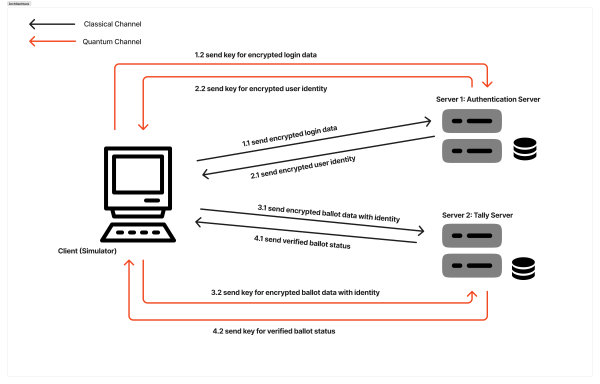
\includegraphics{Auth-Tally2.png}
\end{center}
\caption[Poem]{ภาพรวมและลำดับขั้นตอนของการดำเนินการโหวต}
\label{fig:auth-tally}
\end{figure}

\subsection{เซิร์ฟเวอร์ยืนยันตัวตัน (Authentication Server)}
เซิร์ฟเวอร์ยืนยันตัวตน (Authentication Server) จะเก็บข้อมูลของผู้มีสิทธิ์โหวตทุกคน ว่ามีใครบ้าง และเก็บลักษณะเฉพาะตัว (identity) ของบัตรเลือกทุกใบตั้งไว้ 
ผู้มีสิทธิ์โหวตจะทำการยืนยันตัวตนกับเซิร์ฟเวอร์ยืนยันตัวตนก่อนทำการโหวต โดยการส่งข้อมูลส่วนตัวของตัวเองให้กับเซิร์ฟเวอร์ 
เมื่อเซิร์ฟเวอร์ทำการตรวจสอบและพบว่า ผู้ใช้มีชื่ออยู่ในผู้มีสิทธิ์ จะทำการส่งลักษณะเฉพาะตัว (identity) ของบัตรลงคะแนนกลับไปให้กับผู้มีสิทธิ์โหวต

กระบวนการที่ผู้มีสิทธิ์โหวตส่งข้อมูลส่วนตัวเพื่อรับการยืนยันตัวตน และการที่เซิร์ฟเวอร์ส่งลักษณะเฉพาะตัวของบัตรลงคะแนนกลับมาให้ผู้มีสิทธิ์โหวต 
จะดำเนินการส่งโดยใช้การกระจายคีย์แบบควอนตัม เพื่อรับประกันความปลอดภัยของการส่งข้อมูล

\subsection{เซิร์ฟเวอร์นับและจัดเก็บผลโหวต (Tally Server)}
เซิร์ฟเวอร์นับและจัดเก็บผลโหวต (Tally Server) จะคอยรับบัตรลงคะแนนออนไลน์จากผู้มีสิทธิ์โหวต โดยเซิร์ฟเวอร์ดังกล่าวจะจดจำลักษณะเฉพาะตัวของบัตรลงคะแนนทุกใบได้
ผู้โหวต นอกจากจะต้องแนบผลการตัดสินใจโหวตจะต้องยืนยันตัวตน และทำการแนบลักษณะเฉพาะตัวของบัตรลงคะแนน (identity) มาพร้อมกับผลการโหวตด้วย 
เซิร์ฟเวอร์สำหรับนับและจัดเก็บผลโหวต จะตรวจสอบลักษณะเฉพาะตัวว่าถูกต้องหรือไม่ ถ้าลักษณะเฉพาะตัวไม่ถูกต้อง เซิร์ฟเวอร์จะทำการปฏิเสธบัตรลงคะแนนดังกล่าว
แต่ถ้าลักษณะเฉพาะตัวของบัตรลงคะแนนถูกต้อง จะทำการบันทึกผลการโหวต และทำการระบุว่าลักษณะเฉพาะตัวดังกล่าว ได้ถูกนำไปใช้ในการโหวตแล้ว

เนื่องจากผู้มีสิทธิ์โหวต มีลักษณะเฉพาะตัวของบัตรลงคะแนนไว้กับตัวเอง จึงสามารถเก็บไว้ และสอบถามเซิร์ฟเวอร์นับและจัดเก็บผลโหวตได้ว่า ลักษณะเฉพาะตัวที่ตัวเองเก็บไว้
ได้ถูกใช้ในการโหวตหรือยัง ใช้ในการโหวตตัวเลือกอะไร เพื่อยืนยันความถูกต้องของผลการโหวตได้

กระบวนการส่งข้อมูลการโหวต จะดำเนินการส่งโดยใช้การกระจายคีย์แบบควอนตัม เพื่อรับประกันความปลอดภัยของการส่งข้อมูล


\section{ฟังก์ชันการทำงานของระบบจำลองการโหวต}

ระบบจำลงการโหวตโดยใช้การกระจายคีย์แบบควอนตัม 
ทำการออกแบบให้อยู่ในระบบของ Web Application เพื่อลดความซ้ำซ้อนในการดาวน์โหลดซอฟต์แวร์เพิ่มเติมลงในอุปกรณ์ของผู้ที่สนใจ
และยังทำให้ระบบจำลองเข้าถึงง่ายจากผู้มีส่วนได้ส่วนเสีย ระบบจะมีฟังก์ชันการทำงานทั้งหมดดังนี้



\subsection{ระบบส่งข้อมูลด้วย BB84}
  เป็นฟังก์ชันหลักของระบบจำลองการโหวต โดยจะจำลองการส่งข้อมูลระหว่างผู้มีสิทธิ์โหวต เซิร์ฟเวอร์ยืนยันตัวตน และเซิร์ฟเวอร์นับและจัดเก็บผลโหวต 
โดยใช้ระบบกระจายคียร์แบบควอมตัม และจำลองให้มีผู้ดักฟังคอยตรวจสอบผลการโหวต หลังจากเสร็จสิ้นขั้นตอนการโหวต ระบบจะแสดงผลว่าการจัดส่งข้อมูลด้วยการกระจายคีย์แบบควอนตัม ภายใต้ Protocol BB84 
มีอัตราการตรวจจับการดักฟังสำเร็จในแต่ละขั้นตอน ดังนี้

1. อัตราการตรวจสอบการดักฟังสำเร็จสำหรับขั้นตอนการส่งข้อมูลยืนยันตัวตน 

2. อัตราการตรวจสอบการดักฟังสำเร็จหรับขั้นตอนการส่งเอกลักษณ์ของบัตรลงคะแนน

3. อัตราการตรวจสอบการดักฟังสำเร็จสำหรับขั้นตอนการส่งผลการโหวตไปยังเซิร์ฟเวอร์

\subsection{ระบบยืนยันความถูกต้องของผลการโหวตโดยการใช้เอกลักษณ์ของบัตรลงคะแนน (identity)}
  ระบบจำลองสามารถให้ผู้มีสิทธิ์โหวต ตรวจสอบได้ว่าทำการโหวตอะไรไปกับเซิร์ฟเวอร์ โดยการแนบเอกลักษณ์ของบัตรลงคะแนน
ไปให้กับเซิร์ฟเวอร์ และเซิร์ฟเวอร์นับและจัดเก็บผลโหวต จะทำการส่งผลการโหวตมาให้ผู้มีสิทธิ์โหวต เพื่อเป็นการยืนยันความถูกต้องของสิ่งที่ผู้มีสิทธิ์โหวตได้ทำการเลือก

  ระบบจะแสดงผลการโหวตของผู้มีสิทธิ์โหวตคนดังกล่าว และจำลองการดักฟังข้อมูลในขั้นตอนของการสื่อสารทั้งหมด
และแสดงอัตราการตรวจสอบการดักฟังสำเร็จดังนี้

1. อัตราการตรวจสอบการดักฟังสำเร็จสำหรับขั้นตอนการส่งเอกลักษณ์ของบัตรลงคะแนน

2. อัตราการตรวจสอบการดักฟังสำเร็จสำหรับการส่งผลการโหวตให้กับผู้มีสิทธิ์โหวต

\subsection{ระบบปรับเปลี่ยนความยาวของคีย์ในการเข้ารหัสข้อมูล}
  ระบบจำลอง สามารถให้ผู้ใช้งานระบบจำลอง กำหนดความยาวของคีย์ในการเข้ารหัสข้อมูล โดยสามารถกำหนดได้ตั้งแต่
ความยาว 0.5 เท่าของขนาดข้อความ ไปจนถึง 6 เท่าของขนาดข้อความ เพื่อตรวจสอบว่ากระทบอัตราการตรวจสอบการดักฟังสำเร็จในขั้นตอนต่างๆอย่างไร


\section{โครงสร้างของระบบจำลองการโหวต}
องค์ประกอบทั้งหมดของระบบจำลองการโหวตที่เป็น Web Application สามารถแบ่งได้ดังนี้

\subsection{ส่วนติดต่อผู้ใช้งาน (User Interface)}
เป็นส่วนที่ผู้ใช้งาน สามารถกำหนดค่า และเลือกใช้ฟีเจอร์ต่างๆของระบบจำลองการโหวต

ออกแบบหน้าตาส่วนติดต่อผู้ใช้งานผ่านโปรแกรม Figma และ
พัฒนาโดยใช้โดยใช้ภาษา Typescript บนเฟรมเวิร์ค Vite โดยมีไลบรารีหลักคือ React

\subsection{ส่วนประมวลผลการทำงาน (Server)}
เป็นส่วนที่คอยประมวลผลการทำงานของระบบจำลองผลการโหวต รับการกำหนดค่า และฟังก์ชันการทำงานที่สนใจจากผู้ใช้
แล้วส่งข้อมูลอัตราการตรวจสอบการดักฟังสำเร็จกลับไปหาส่วนติดต่อผู้ใช้งาน

พัฒนาโดยใช้ภาษา Python บนเฟรมเวิร์ค FastAPI สำหรับการส่งข้อมูลไปยังส่วนติดต่อผู้ใช้งาน
มีไลบรารีหลักที่เกี่ยวข้องคือ Qiskit IBM Runtime ขององค์กร IBM Quantum 
สำหรับการเขียนโปรแกรม Quantum Assembly และส่งให้ควอนตัมคอมพิวเตอร์ของ IBM ทำการจำลองการส่งข้อมูลด้วยการกระจายคีย์แบบควอนตัม และส่งผลลัพธ์กลับมาหาส่วนประมวลผลการทำงาน

\subsection{ส่วนฐานข้อมูล (Database)}
เป็นส่วนที่จัดเก็บข้อมูลต่างๆในระบบจำลอง ได้แก้ รายชื่อผู้มีสิทธิ์โหวต รายการของเอกลักษณ์ของบัตรลงคะแนนเสียงแต่ละใบ 
และการกำหนดค่าสำหรับระบบจำลองข้อผู้ใช้แต่ละคน และคอยส่งข้อมูลดังกล่าวให้กับส่วนประมวลผลการทำงาน เมื่อมีการร้องข้อ

เลือกใช้ MongoDB ซึ่งเป็น NoSQL สำหรับการจัดเก็บข้อมูลเนื่องจากสามารถจัดเก็บข้อมูลได้เยอะ มีโครงสร้างการจัดเก็บข้อมูลที่ยืดหยุ่นและปรับได้ตลอดเวลา
ซึ่งเหมาะสำหรับการเก็บรายชื่อผู้มีสิทธิ์โหวต และเอกลักษณ์ของบัตรลงคะแนนแต่ละใบ เนื่องจากมีโครงสร้างที่อาจปรับเปลี่ยนได้ และมีจำนวนข้อมูลมหาศาล


\chapter{\ifproject%
\ifenglish Experimentation and Results\else การทดลองและผลลัพธ์\fi
\else%
\ifenglish System Evaluation\else การประเมินระบบ\fi
\fi}

ในบทนี้จะทดสอบเกี่ยวกับการทำงานในฟังก์ชันหลัก ๆ ของระบบ ทั้งในระดับการจำลอง (Simulation) และการพัฒนาเชิงต้นแบบ (Prototype)

\section{วัตถุประสงค์ของการประเมินระบบ}

การประเมินระบบในโครงงานนี้มีวัตถุประสงค์เพื่อจำลองการทำงานและแสดงแนวคิดเชิงปฏิบัติ (Proof of Concept) ของระบบโหวตความปลอดภัยสูงที่ใช้เทคโนโลยี Quantum Key Distribution (QKD) และ Blind Signature

นอกจากนี้ โครงงานยังมีการพัฒนาในระดับ implementation เบื้องต้น เพื่อแสดงให้เห็นว่าระบบสามารถนำไปใช้งานได้จริงในบางส่วน โดยมุ่งเน้นการทดสอบกลไกหลักของระบบ เช่น การเข้ารหัส การแจกจ่ายกุญแจ และกระบวนการโหวต

การประเมินจะครอบคลุมในประเด็นต่อไปนี้

\begin{itemize}
    \item ความเป็นไปได้ของการใช้ QKD ในการแจกจ่ายกุญแจสำหรับระบบโหวต
    \item ความสามารถของ Blind Signature ในการรักษาความเป็นนิรนามของผู้โหวต
    \item ความถูกต้องของกระบวนการโหวตภายใต้การจำลอง
    \item การแสดงให้เห็นถึงความปลอดภัยของระบบในเชิงแนวคิด
\end{itemize}

\section{ขอบเขตการทดสอบ}

การประเมินระบบแบ่งออกเป็น 2 ส่วนหลัก ได้แก่

\subsection{Simulation Level}

\begin{itemize}
    \item จำลองกระบวนการ QKD (BB84 protocol)
    \item จำลองการตรวจจับการดักฟัง (Eavesdropper)
    \item จำลองการเข้ารหัสและถอดรหัสข้อมูล
    \item จำลองการทำ Blind Signature
\end{itemize}

\subsection{Implementation Level (Prototype)}

\begin{itemize}
    \item พัฒนาระบบโหวตต้นแบบ (เช่น web-based หรือ script)
    \item ทดสอบการส่งข้อมูลโหวตจริงผ่านระบบ
    \item ทดสอบการใช้งานของผู้ใช้ในสถานการณ์จำลอง
\end{itemize}

\section{วิธีการทดสอบ}

\subsection{การทดสอบความถูกต้อง (Functional Testing)}

ทำการทดสอบการทำงานของระบบในแต่ละขั้นตอน เช่น การโหวต การเข้ารหัส และการถอดรหัสข้อมูล เพื่อให้แน่ใจว่าระบบทำงานได้ถูกต้องตามที่ออกแบบไว้

\subsection{การทดสอบความปลอดภัย (Security Testing)}

ทดสอบการป้องกันการโจมตี เช่น

\begin{itemize}
    \item การดักฟังข้อมูล (Eavesdropping)
    \item การปลอมแปลงข้อมูล (Tampering)
    \item การโจมตีแบบ Man-in-the-Middle
\end{itemize}

โดยใช้คุณสมบัติของ QKD ที่สามารถตรวจจับการดักฟังได้
\ifproject
\include{chapters/conclusion}
\fi

\bibliography{sampleReport}

\ifproject
\normalspacing
\appendix
\include{chapters/appendix}

%% Display glossary (optional) -- need glossary option.
\ifglossary\glossarypage\fi

%% Display index (optional) -- need idx option.
\ifindex\indexpage\fi

\begin{biosketch}
\begin{center}
  \includegraphics[width=1.5in]{mugshot.jpg}
\end{center}
Your biosketch goes here. Make sure it sits inside
the \texttt{biosketch} environment.
\end{biosketch}
\fi % \ifproject
\end{document}
